\documentclass[aspectratio=169,14pt]{beamer}
\usetheme{Madrid}
\usepackage{graphicx}
\usepackage{xcolor}

\definecolor{reapblue}{RGB}{29,78,216}
\definecolor{reapgreen}{RGB}{21,128,61}
\definecolor{reapamber}{RGB}{161,98,7}
\definecolor{reapgrey}{RGB}{226,232,240}

\setbeamercolor{frametitle}{bg=reapblue,fg=white}
\setbeamercolor{title}{bg=reapblue,fg=white}
\setbeamerfont{frametitle}{size=\LARGE,series=\bfseries}
\setbeamerfont{itemize/enumerate body}{size=\normalsize}
\setbeamerfont{itemize/enumerate subbody}{size=\normalsize}
\setbeamertemplate{itemize item}{\color{reapblue}\Large$\bullet$}
\setbeamertemplate{navigation symbols}{}

% progress bar: \pbar{<filled cm>}{<label>}
\newcommand{\pbar}[2]{%
  {\color{reapgreen}\rule{#1}{10pt}}{\color{reapgrey}\rule{\dimexpr6cm-#1\relax}{10pt}}~~\large #2%
}

\title{R.E.A.P : Realtime Edge Agentic Physio-Buddy}
\subtitle{Progress Update --- October done, November started}
\author{Shishir SH (231IT067) \and Rahul S (231IT054) \and Ashab M (231IT011)}
\institute{NITK Surathkal \quad\textbar\quad Guide: Prof.\ Ram Mohana Reddy Guddeti}
\date{October 2026}

\begin{document}

% 1 ---- title ----
\begin{frame}
  \titlepage
\end{frame}

% 2 ---- problem ----
\begin{frame}{Problem: form fails before you feel it}
  \begin{itemize}
    \item \textbf{Silent breakdown:} posture worsens before you feel tired.
    \item \textbf{Real danger:} bad form strains joints --- worst for older adults.
    \item \textbf{No coach:} you cannot watch yourself mid-exercise.
    \item \textbf{Our answer:} a phone buddy that watches and speaks up each rep.
  \end{itemize}
\end{frame}

% 3 ---- milestones ----
\begin{frame}{Where we stand on the timeline}
  \begin{itemize}
    \item September --- body tracking \hfill \textbf{done}
    
    \pbar{6cm}{100\%}
    \medskip
    \item October --- workout framework \hfill \textbf{done}
    
    \pbar{6cm}{100\%}
    \medskip
    \item November --- lightweight on-device mode \hfill \textbf{starter}
    
    \pbar{1.8cm}{30\%}
  \end{itemize}
\end{frame}

% 4 ---- October work ----
\begin{frame}{October is done: the workout framework}
  \begin{columns}[T]
    \begin{column}{0.47\textwidth}
      \setlength{\itemsep}{3pt}
      \begin{itemize}
        \item \textbf{3 exercise guides,} each with a healthy bend range.
        \item \textbf{Automatic rep counting} that ignores small wobbles.
        \item Coaching message after every rep.
      \end{itemize}
    \end{column}
    \begin{column}{0.50\textwidth}
      \centering
      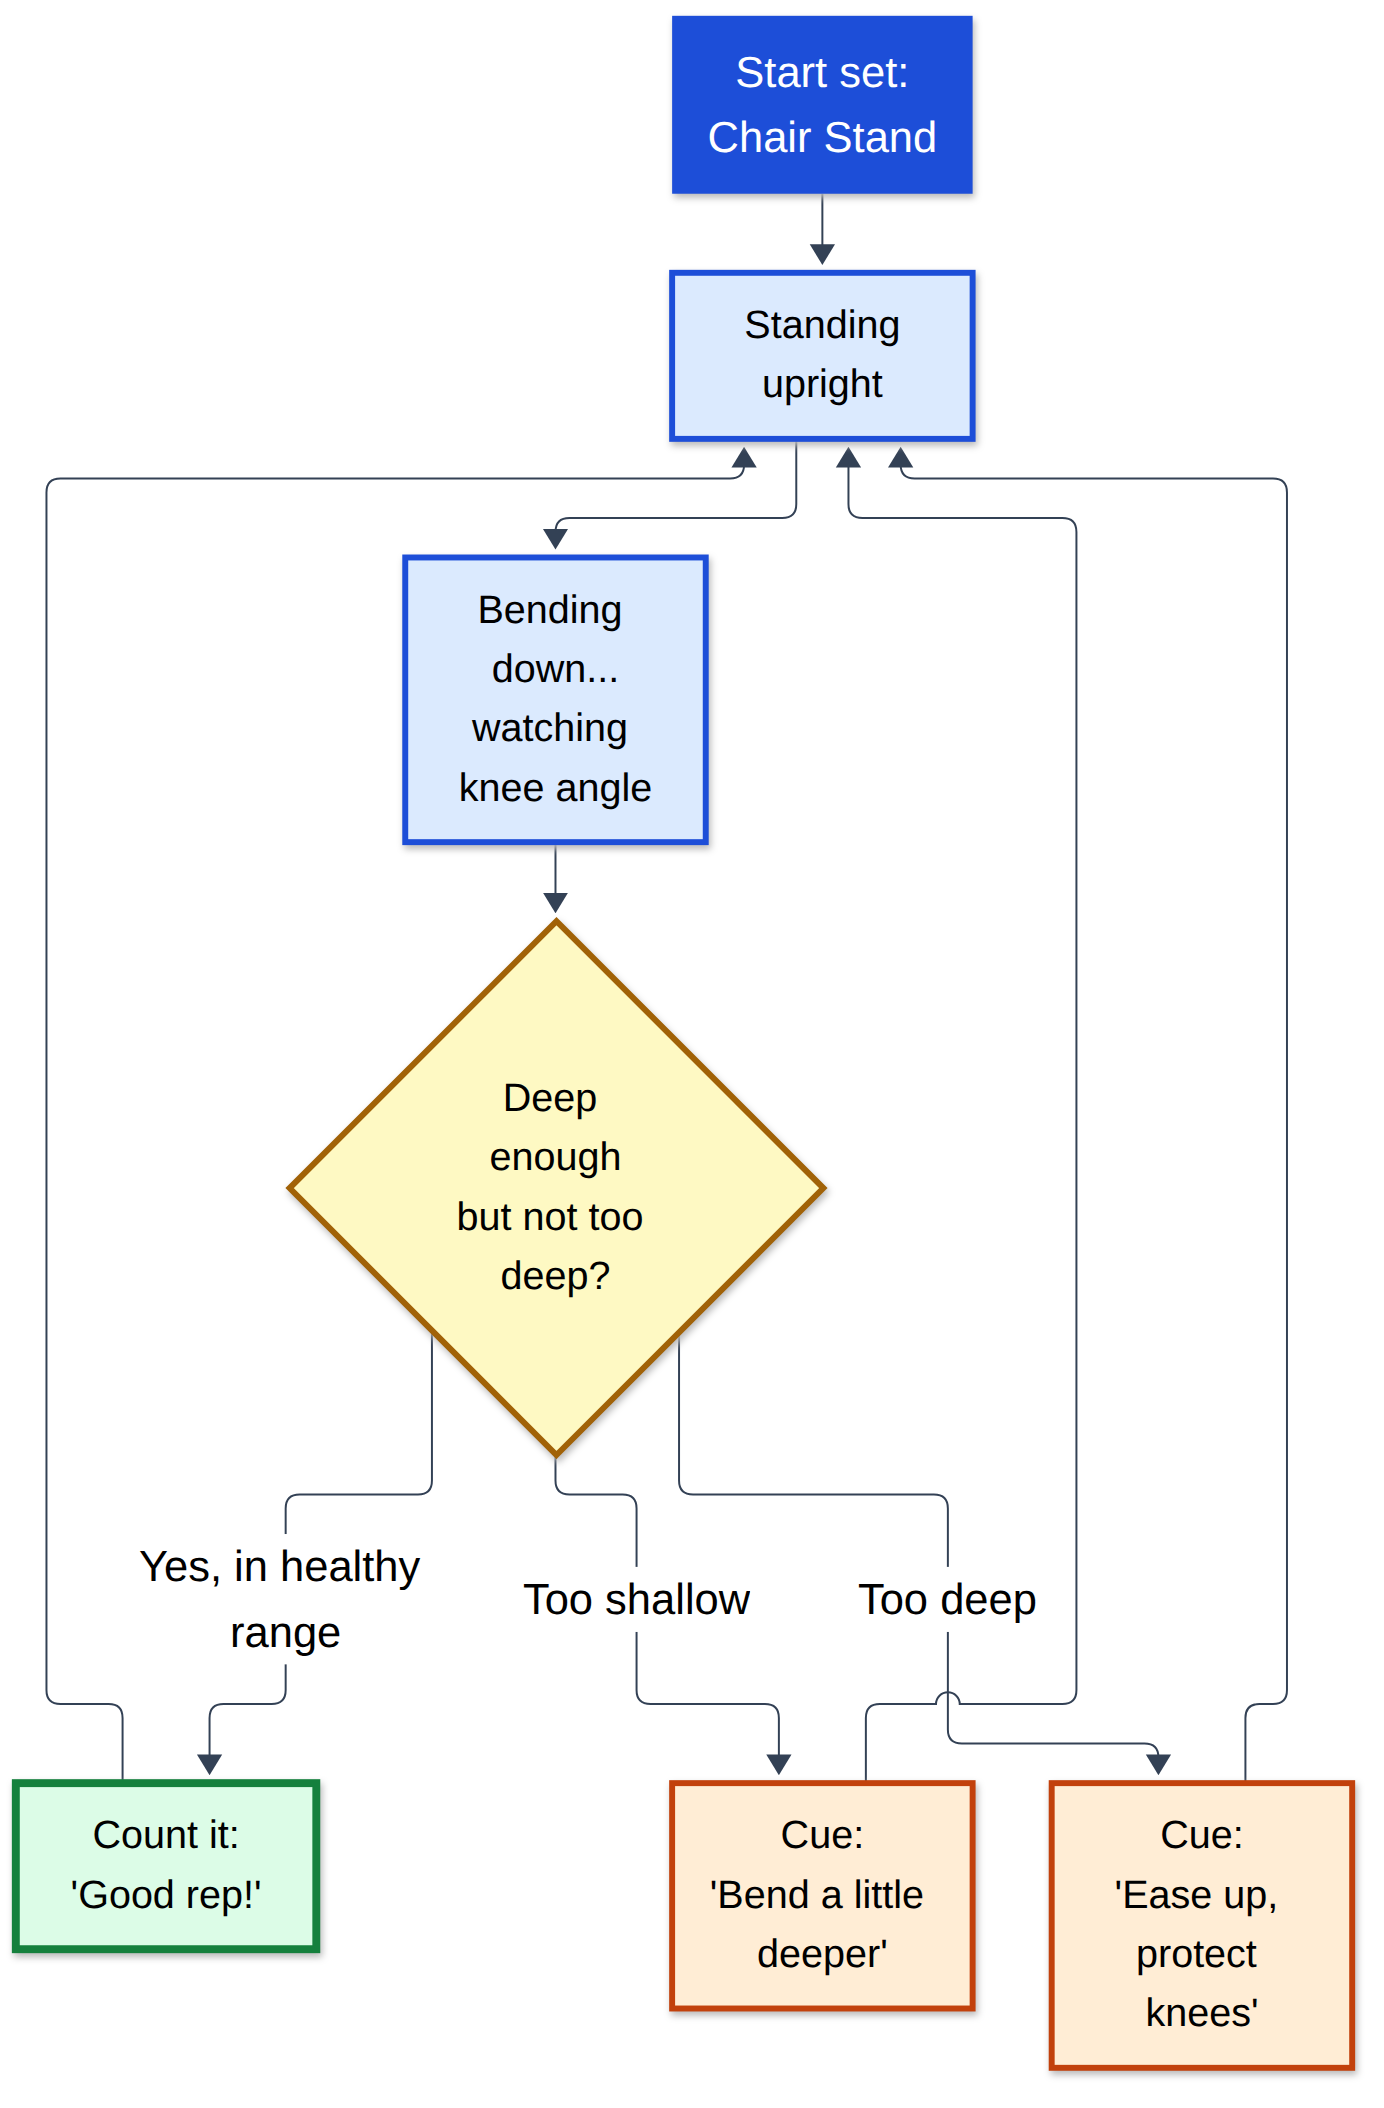
\includegraphics[width=\textwidth,height=0.60\textheight,keepaspectratio]{diagrams/d2_session.png}
    \end{column}
  \end{columns}
\end{frame}

% 5 ---- system view ----
\begin{frame}{How the whole buddy fits together}
  \centering
  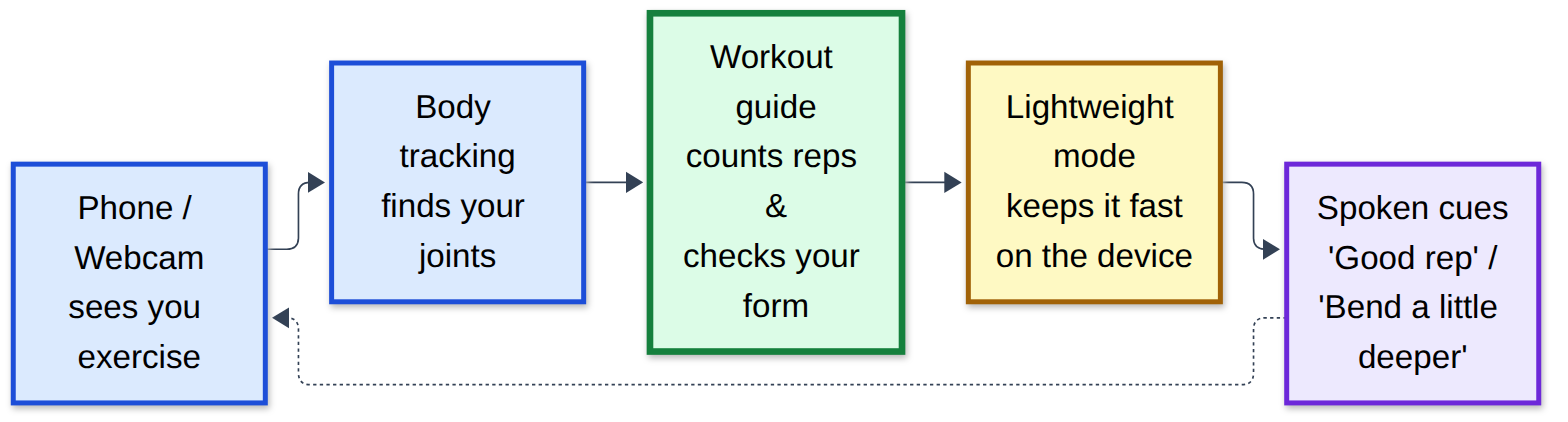
\includegraphics[width=0.96\textwidth,keepaspectratio]{diagrams/d1_pipeline.png}
  
  \large Everything runs on the device itself --- no internet needed mid-set.
\end{frame}

% 6 ---- November starter ----
\begin{frame}{November starter (30\%): lightweight mode}
  \begin{columns}[T]
    \begin{column}{0.47\textwidth}
      \setlength{\itemsep}{3pt}
      \begin{itemize}
        \item \textbf{Lite mode:} smaller picture, every other frame.
        \item \textbf{Built-in stopwatch} logs time spent per frame.
        \item Plain-words alert when the phone runs slow.
      \end{itemize}
    \end{column}
    \begin{column}{0.50\textwidth}
      \centering
      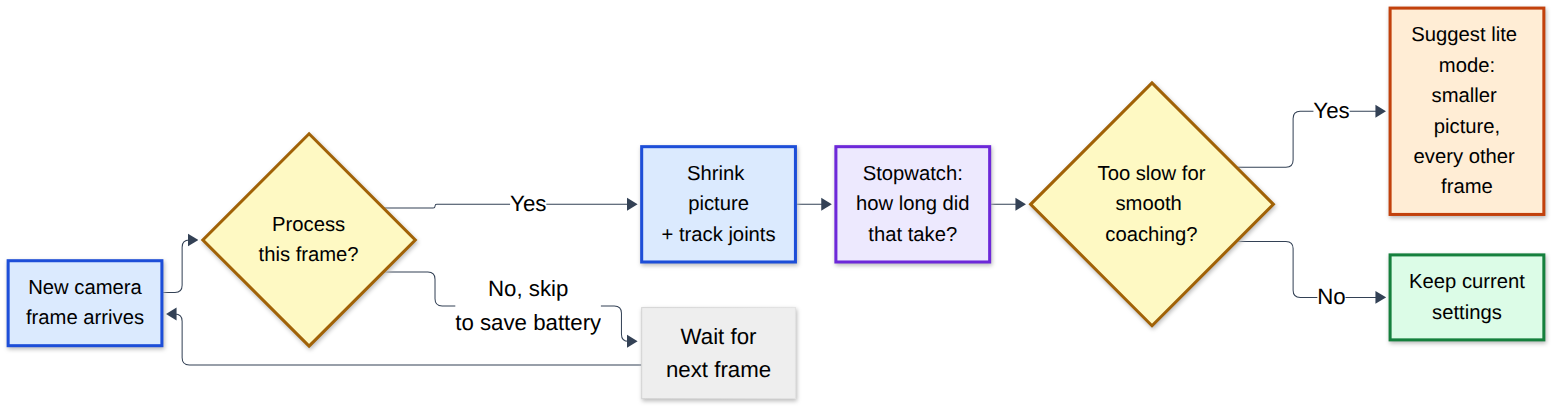
\includegraphics[width=\textwidth,keepaspectratio]{diagrams/d3_edge.png}
    \end{column}
  \end{columns}
\end{frame}

% 7 ---- one rep flow ----
\begin{frame}{One rep, in under a second}
  \centering
  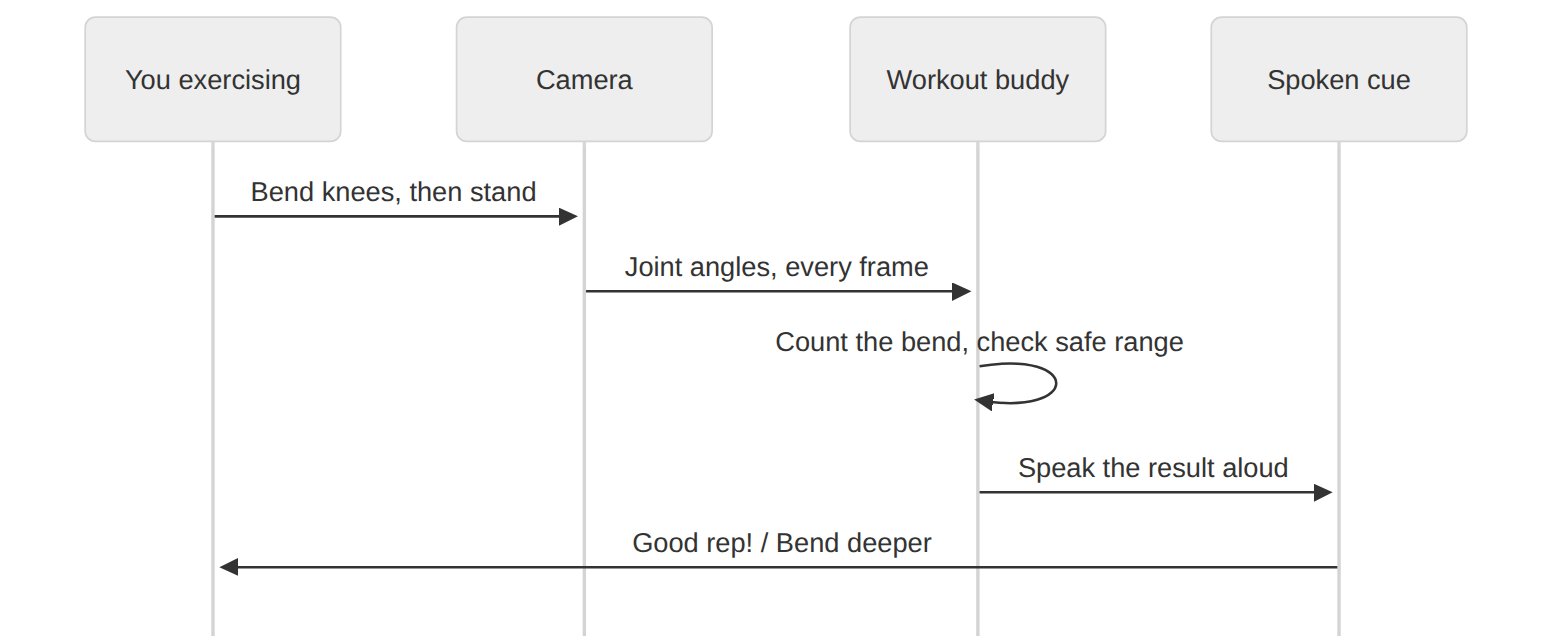
\includegraphics[width=0.92\textwidth,keepaspectratio]{diagrams/d5_sequence.png}
  
  \large Bend, check, speak --- all before the next rep starts.
\end{frame}

% 8 ---- next work ----
\begin{frame}{Next work}
  \begin{columns}[T]
    \begin{column}{0.55\textwidth}
      \begin{itemize}
        \item Finish lite mode (remaining 70\%): faster models, battery testing.
        \medskip
        \item December: voice engine that \textbf{speaks cues aloud} on-device.
        \medskip
        \item Then: test everything on \textbf{real recorded exercises}.
      \end{itemize}
    \end{column}
    \begin{column}{0.40\textwidth}
      \centering
      {\LARGE\bfseries\color{reapblue} Thank you!}\\[1ex]
      {\large Questions welcome.}
    \end{column}
  \end{columns}
\end{frame}

\end{document}
